\section{Data Description and Preparation}

\subsection{Source and Context}
We use the Health Behaviour in School-aged Children (HBSC) dataset from 2018, a WHO-supported cross-national survey that collects health-related data from adolescents aged 11, 13, and 15. It includes data on well-being, social relationships, behaviours, and demographic characteristics across more than 40 countries. The dataset contains 120 variables.

\subsection{Missing Data}
In the appendix, the number of missing values coded as sysmiss and represented as Nones in the dataset is shown. Besides that, there are also more types of missingness observed in data, such as "Missing due to skip pattern"(99) or "Missing due to inconsistent answer"(-99).

\begin{tabular}{lrrrrrrr}
\toprule
talkstepfa & 0.000000 & 1.000000 & 2.000000 & 3.000000 & 4.000000 & 5.000000 & Total \\
talkfather &  &  &  &  &  &  &  \\
\midrule
0.000000 & 2712 & 267 & 389 & 252 & 146 & 1487 & 5253 \\
1.000000 & 20628 & 4954 & 2997 & 2028 & 1247 & 41923 & 73777 \\
2.000000 & 18105 & 944 & 4816 & 3012 & 1582 & 49887 & 78346 \\
3.000000 & 7975 & 503 & 1438 & 3269 & 1627 & 25477 & 40289 \\
4.000000 & 3322 & 302 & 599 & 679 & 2714 & 11394 & 19010 \\
5.000000 & 2045 & 921 & 1661 & 1087 & 1311 & 8159 & 15184 \\
Total & 54787 & 7891 & 11900 & 10327 & 8627 & 138327 & 231859 \\
\bottomrule
\end{tabular}

\begin{tabular}{lrrrrrrr}
\toprule
talkstepmo & 0.000000 & 1.000000 & 2.000000 & 3.000000 & 4.000000 & 5.000000 & Total \\
talkmother &  &  &  &  &  &  &  \\
\midrule
0.000000 & 1749 & 188 & 226 & 149 & 69 & 902 & 3283 \\
1.000000 & 30505 & 5116 & 3667 & 3092 & 2487 & 71032 & 115899 \\
2.000000 & 17244 & 671 & 3755 & 2570 & 1926 & 48747 & 74913 \\
3.000000 & 4830 & 340 & 608 & 1913 & 1107 & 15244 & 24042 \\
4.000000 & 1728 & 181 & 250 & 217 & 1622 & 5278 & 9276 \\
5.000000 & 712 & 368 & 358 & 200 & 203 & 2605 & 4446 \\
Total & 56768 & 6864 & 8864 & 8141 & 7414 & 143808 & 231859 \\
\bottomrule
\end{tabular}


\subsection{Variables Selected}
The \textbf{variables used to calculate the Family Affluence Scale III (FAS III)} are:

\begin{longtable}{@{}ll@{}}
\toprule
\textbf{Variable Name} & \textbf{Description} \\
\midrule
\texttt{fasfamcar} & Does your family own a car, van or truck? \\
\texttt{fasbedroom} & Do you have your own bedroom for yourself? \\
\texttt{fascompu} & Number of computers (PCs, laptops, tablets) in the household \\
\texttt{fasbathr} & Number of bathrooms in the home (with bath or shower) \\
\texttt{fasdishw} & Does your family have a dishwasher? \\
\texttt{fasholid} & How many times did your family travel abroad for holidays last year? \\
\bottomrule
\end{longtable}

These are the six core material affluence indicators retained in the HBSC FAS III scoring system. In addition to these, the dataset includes two computed indicators:
\begin{itemize}
  \item \texttt{IRFAS} – Family Affluence Scale III (continuous score)
  \item \texttt{IRRELFAS} – Relative family affluence category (categorical: low, medium, high)
\end{itemize}

\subsection{Data Issues and Preprocessing}
\begin{itemize}
    \item \textbf{Missing data}: [How you handled NA values - deletion, imputation, etc.]
    \item \textbf{Data types}: [How categorical variables were encoded - label encoding, discretization]
    \item \textbf{Sample size}: [Number of observations after cleaning]
\end{itemize}

% \subsection{Scientific Question}
% Relationship of social integration of a child and aggression levels channeled through bullying and participation in fights.

% \begin{figure}[h]
%     \centering
%     \begin{subfigure}[t]{0.48\textwidth}
%         \centering
%         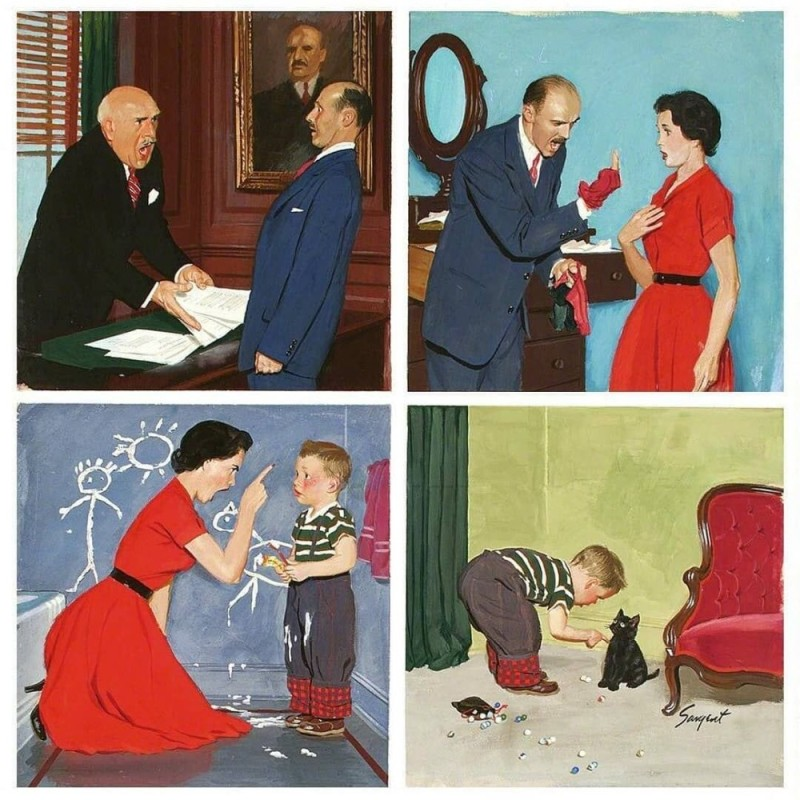
\includegraphics[width=\textwidth]{Report/pics/cycle of abuse.png}
%         \caption{Inspirational diagram for forming a scientific question.}
%     \end{subfigure}
%     \hfill
%     \begin{subfigure}[t]{0.48\textwidth}
%         \centering
%         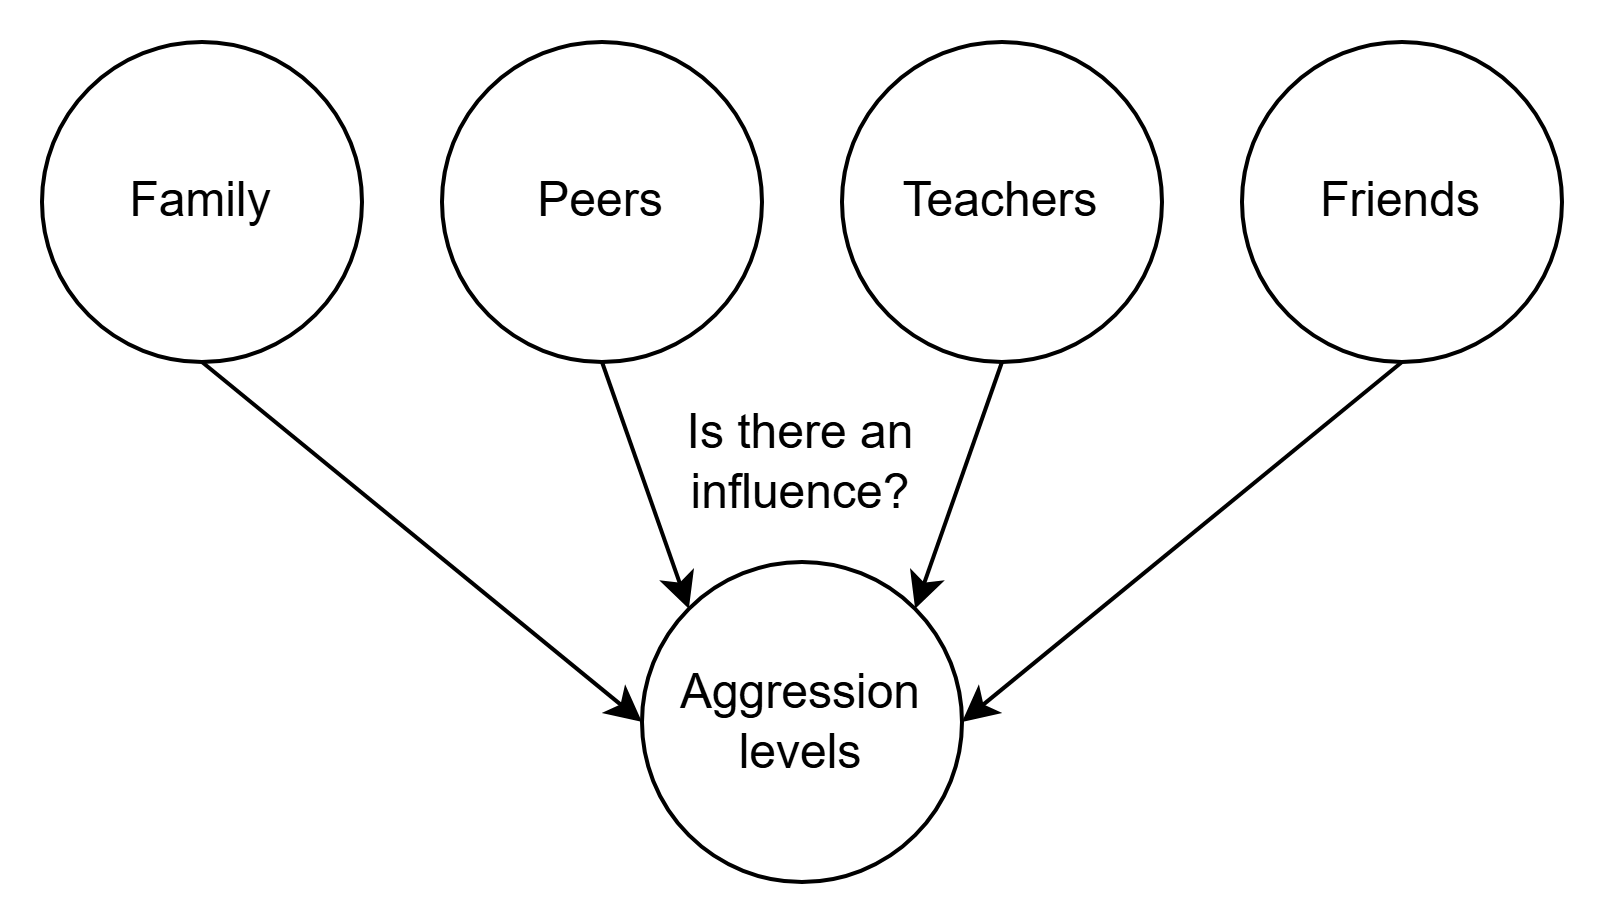
\includegraphics[width=\textwidth]{Report/pics/scheme for scientific question.png}
%         \caption{Conceptual scheme illustrating the scientific question.}
%     \end{subfigure}
%     \caption{The first figure serves as inspiration, while the second is a vague schematic formulation of our scientific question.}
% \end{figure}
